% Source: 2006浙江文.pdf, source-relative PDF page 1, Q14.
% The interior label is B' in the scan; the alpha plane and dashed edges are retained.
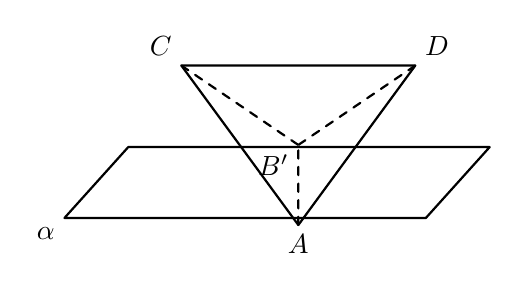
\begin{tikzpicture}[line cap=round,line join=round,x=0.9cm,y=0.9cm]
  \coordinate (C) at (0,2.5);
  \coordinate (D) at (3.3,2.5);
  \coordinate (A) at (1.65,0.25);
  \coordinate (Bp) at (1.65,1.38);
  \coordinate (L) at (-0.75,1.35);
  \coordinate (R) at (4.35,1.35);
  \coordinate (Lb) at (-1.65,0.35);
  \coordinate (Rb) at (3.45,0.35);
  \draw[thick] (L)--(R)--(Rb)--(Lb)--cycle;
  \draw[thick] (C)--(D) (C)--(A) (D)--(A);
  \draw[thick,dashed] (C)--(Bp) (D)--(Bp) (A)--(Bp);
  \node[above left] at (C) {$C$};
  \node[above right] at (D) {$D$};
  \node[below] at (A) {$A$};
  \node[below left] at (Bp) {$B'$};
  \node[below left] at (Lb) {$\alpha$};
\end{tikzpicture}
